\begin{comment}
\documentclass[10pt]{article}
\usepackage{fullpage, graphicx, url}
\setlength{\parskip}{1ex}
\setlength{\parindent}{0ex}
\title{xadsr}
\begin{document}


\begin{tabular}{ccc}
The Alternative Csound Reference Manual & & \\
Previous & &Next

\end{tabular}

%\hline 
\end{comment}
\section{xadsr}
xadsr�--� Calculates the classical ADSR envelope. \subsection*{Description}


  Calculates the classical ADSR envelope 
\subsection*{Syntax}


 ar \textbf{xadsr}
 iatt, idec, islev, irel [, idel]


 kr \textbf{xadsr}
 iatt, idec, islev, irel [, idel]
\subsection*{Initialization}


 \emph{iatt}
 -- duration of attack phase 


 \emph{idec}
 -- duration of decay 


 \emph{islev}
 -- level for sustain phase 


 \emph{irel}
 -- duration of release phase 


 \emph{idel}
 -- period of zero before the envelope starts 
\subsection*{Performance}


  The envelope is the range 0 to 1 and may need to be scaled further. The envelope may be described as: 


 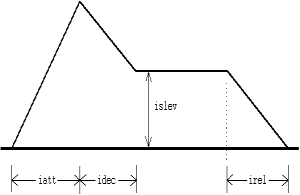
\includegraphics[scale=1]{adsr} 


 Picture of an ADSR envelope.


  The length of the sustain is calculated from the length of the note. This means \emph{adsr}
 is not suitable for use with MIDI events. The opcode \emph{xadsr}
 is identical to \emph{adsr}
 except it uses exponential, rather than linear, line segments. 


 \emph{xadsr}
 is new in Csound version 3.51. 
\subsection*{See Also}


 \emph{adsr}
, \emph{madsr}
, \emph{mxadsr}

%\hline 


\begin{comment}
\begin{tabular}{lcr}
Previous &Home &Next \\
wterrain &Up &xin

\end{tabular}


\end{document}
\end{comment}
